\documentclass[11pt, letterpaper, twoside]{article}
\usepackage[letterpaper, portrait, left=1in, right=1in, top=1in, bottom=1in]{geometry}\usepackage{amsmath}
\usepackage{amssymb}
\usepackage{graphicx}
\usepackage[explicit]{titlesec}
\usepackage{epstopdf}
\usepackage{amsmath}
\usepackage{inputenc}
\usepackage{enumitem}
\usepackage{booktabs, multirow} %for borders and merged ranges
\usepackage{soul}% for underlines
\usepackage[table]{xcolor} % for cell colors
\newcommand\aug{\fboxsep=-\fboxrule\!\!\!\fbox{\strut}\!\!\!} %Use \aug to make a equal column for an augmented matrix. Ie. 1 & 2 & 3 & 4 & \aug & x \\
\begin{document}
\begin{titlepage}
\centering
\vspace*{60px}
\hspace{0pt}

\includegraphics[width=0.2\textwidth]{logo}\par\vspace{1cm}
{\scshape\LARGE Athabasca University \par}
\vspace{1cm}
{\scshape\Large MATH 265\par}
\vspace{1.5cm}
{\huge\bfseries Assignment 3\par}
\vspace{2cm}
{\Large\itshape Stanley Zheng\par}
\vfill
{\large September 3, 2020\par}
\vspace*{50px}
\hspace{0pt}
\pagebreak
\end{titlepage}
\begin{enumerate}
\item \begin{enumerate}[label=(\alph*)] %Question 1
\item Graph of \(f(x)\):

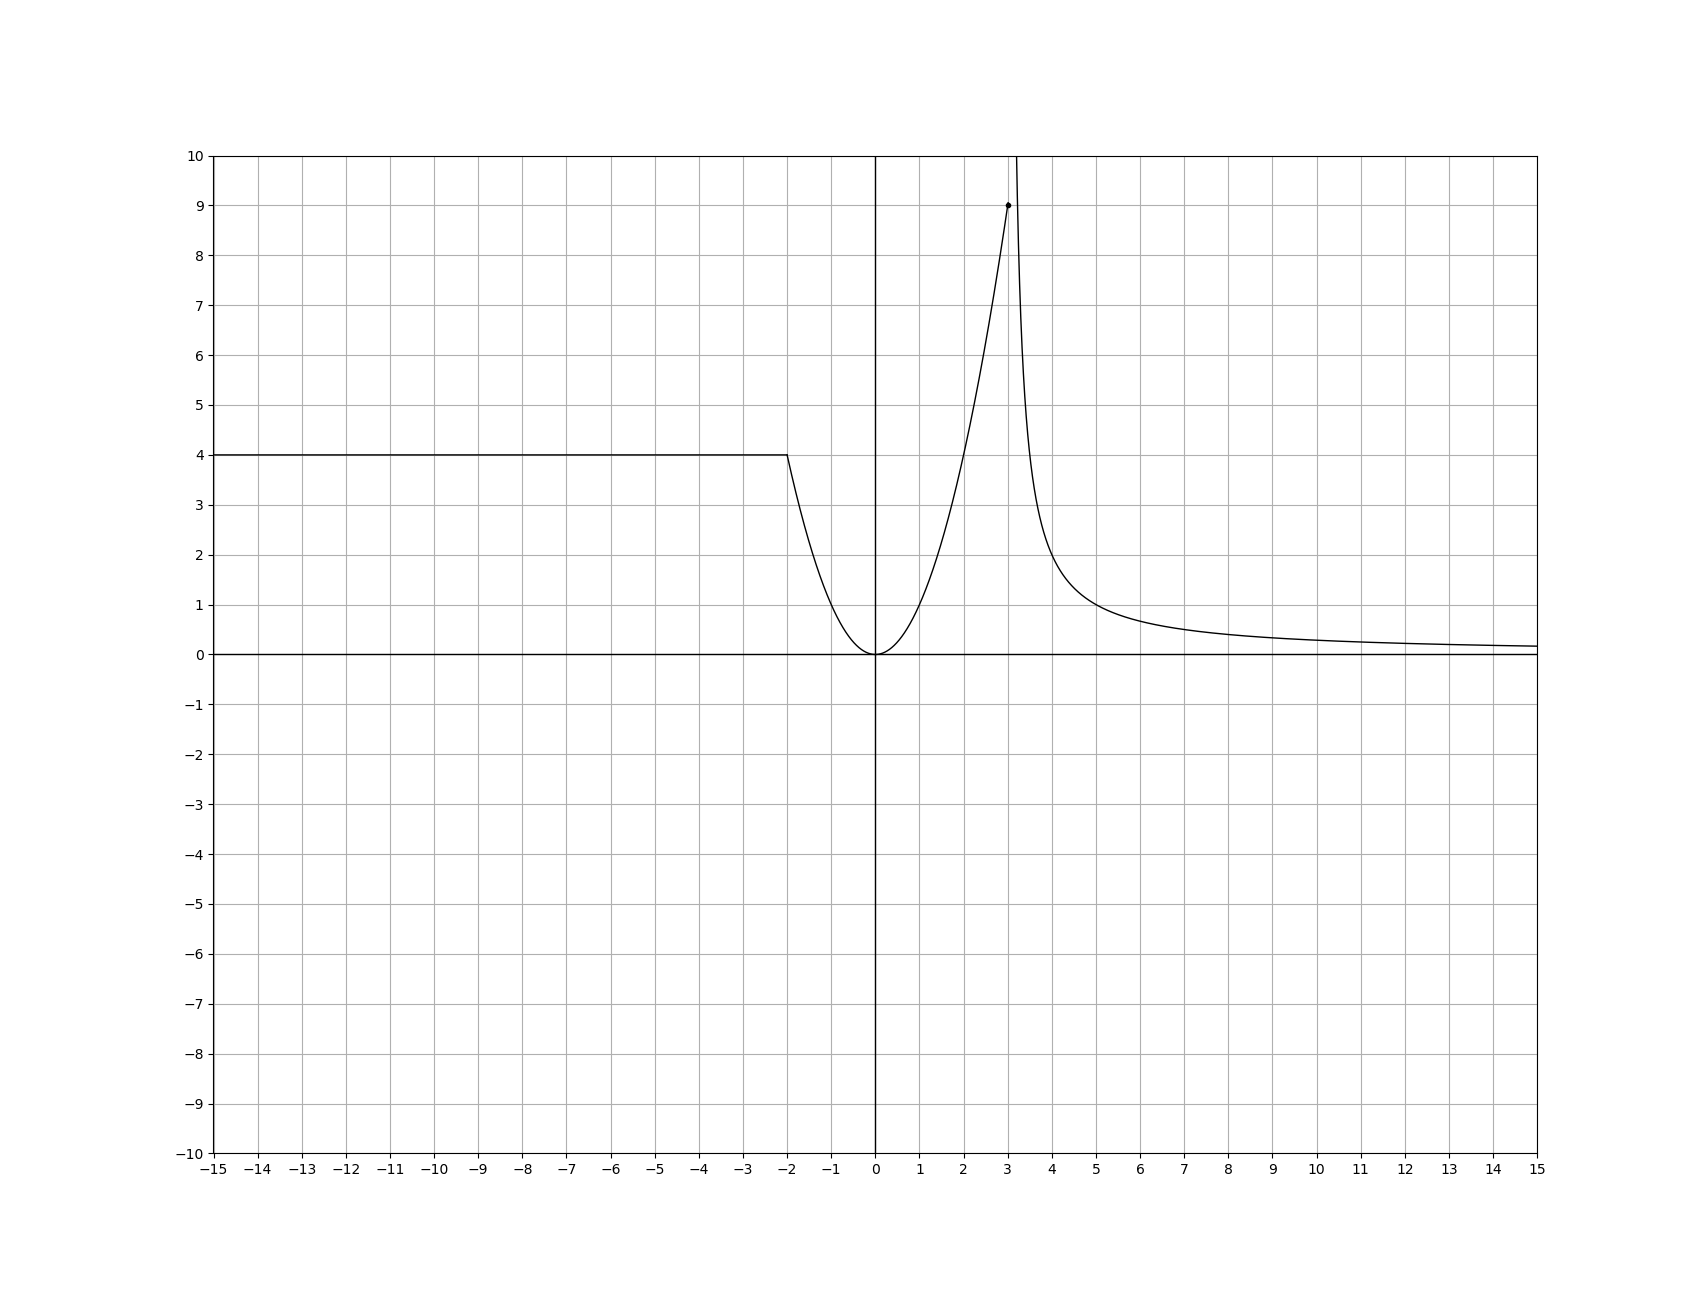
\includegraphics[width=0.85\textwidth]{q1a}

Graph of \(f^\prime(x)\)

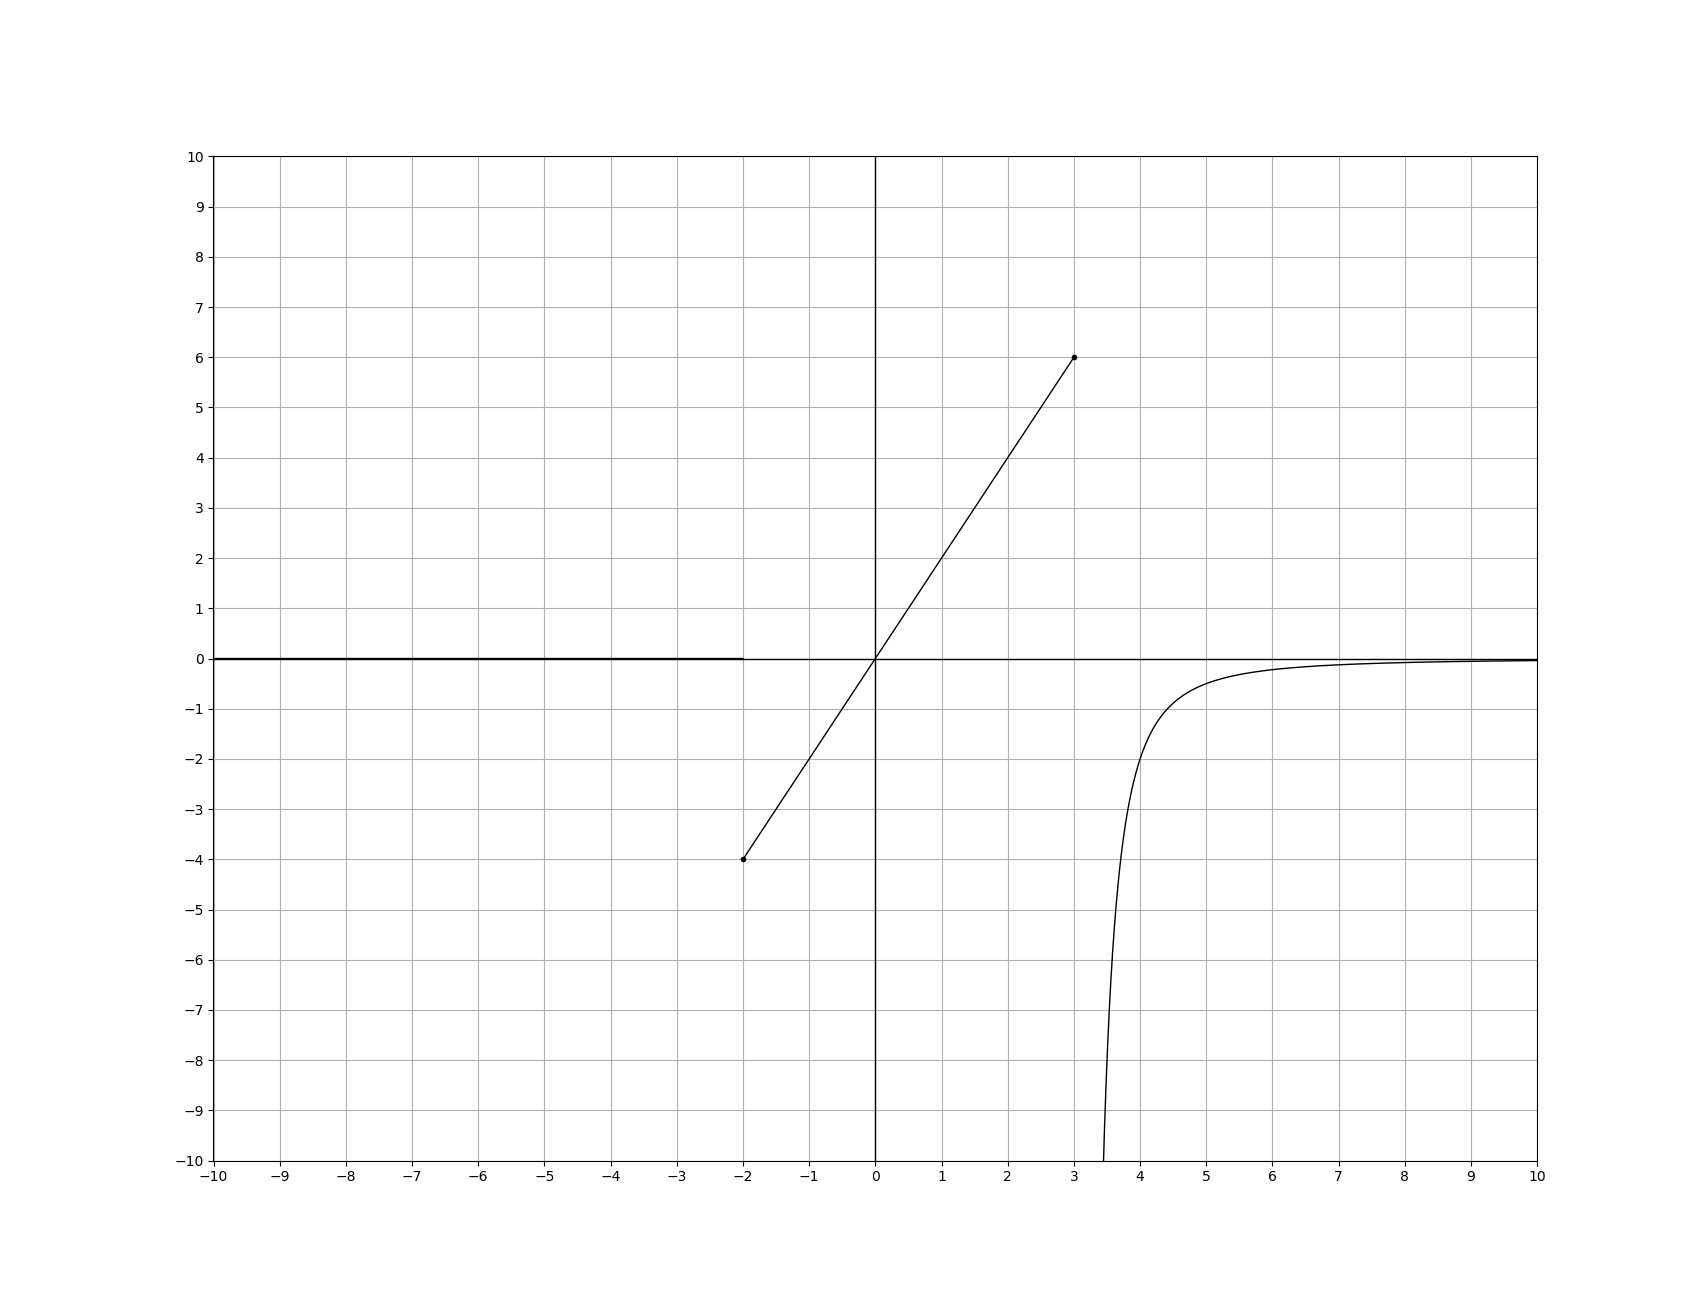
\includegraphics[width=0.85\textwidth]{q2a}

\end{enumerate}
\item \begin{enumerate}[label=(\alph*)]
\item $$\frac{d}{dx}x\cos\sqrt{x-3}=\cos(\sqrt{x-3})-\frac{x\cdot\sin(\sqrt {x-3})}{2\cdot\sqrt{x-3}}$$
\item
\begin{align*}
\frac{d^2}{dx^2}x^2\tan x|_{x=\pi}&=\frac{d}{dx}2x\tan(x)+x^2\sec^2 (x)|_{x=\pi}\\
&=2\tan(x)+2x\sec^2(x)+2x\sec^2(x)+2x^2\sec^2(x)\tan(x)|_{x=\pi}\\
&=2(0)+4\pi+2\pi^2(0)=\boxed{4\pi}
\end{align*}
\item \[\frac{d}{dx}\frac{\sin(x)-\cos(x)}{x^3}=\frac{x(\cos(x)+\sin(x))-3(\sin(x)-\cos(x))}{x^4}\]
\item
\begin{align*}\frac{d}{dx}\frac{f(x)-x^2g(x)}{f(x)+g(x)}|_{x=0}&=\frac{(f(x)-x^2g(x))^\prime(f(x)+g(x))-(f(x)-x^2g(x))(f(x)+g(x))^\prime}{(f(x)+g(x))^2}\\
&=\frac{(f^\prime(x)-x^2g^\prime(x)+2xg(x))(1)-(1-(0)^2(0))(f^\prime(x)+g^\prime(x))}{(1+0))^2}\\
&=\frac{(2-(0^2)(-1)+2(0)(0))-(1)(2+(-1))}{1}\\
&= 1
\end{align*}%CHECK
\end{enumerate}
\item 

Let the distance from home base to first base be \(y\), the distance from first base to the runner be \(x\), and the distance from home plate to the runner be \(z\).

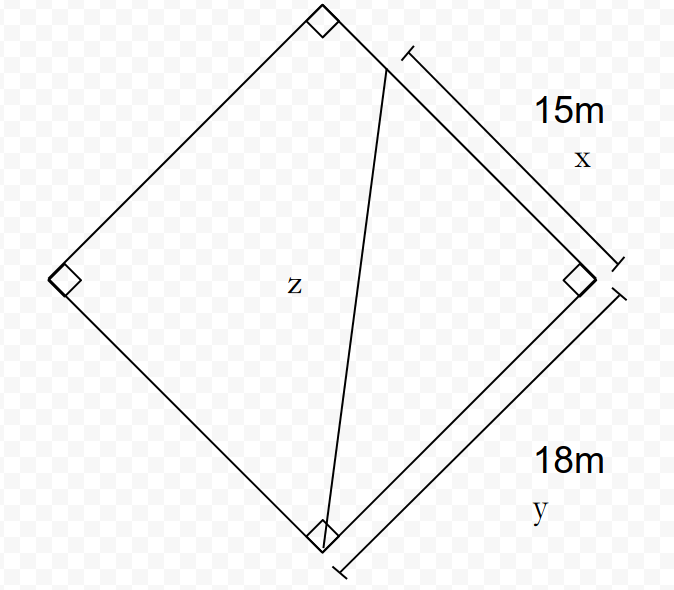
\includegraphics[width=0.4\textwidth]{q3}

We have \(\frac{dt}{dx}=7.5\text{m/s}\). We can also find \(z\) though the pythagorean theorem. \(z^2=18^2+x^2\).

Next we differentiate over \(t\)
\[2z\frac{dz}{dt}=2x\frac{dx}{dt}\]
\[\frac{dz}{dt}=\frac{x}{z}\cdot\frac{dx}{dt}\]
We are given \(x=18-3=15\). Substitute this into the pythagorean theorem to find \(z\)

\[z=\sqrt{18^2+15^2}=3\sqrt{61}.\]

Substituting this back into the derivative, we have

\[\frac{dz}{dt}=\frac{15}{3\sqrt{61}}\cdot7.5=\boxed{4.8m/s}\]

\item \begin{enumerate}[label=(\alph*)]
\item We can first find the derivative of function. \(f(x)=\frac{x-1}{\sqrt{x}}\)

\[f'(x)=\frac{(x-1)^\prime\sqrt{x}-(\sqrt{x}^\prime(x-1))}{(\sqrt{x})^2}\]
\[=\frac{1}{\sqrt{x}}-\frac{x-1}{2x^{\frac{3}{2}}}\]
\[=\frac{2x}{2x^{\frac{3}{2}}}-\frac{x-1}{2x^{\frac{3}{2}}}=\frac{x+1}{2x^{\frac{3}{2}}}\]

Plugging in $x=4$, we have
\[\frac{4+1}{2(4)^{\frac{3}{2}}}=\frac{5}{16}.\]

The \(y\) coordinate is \(f(4)=\frac{3}{2}\). In order for a line with slope \(\frac{5}{16}\) to pass through this point, the \(y\) intercept must be \(\frac{1}{4}\).

Therefore, the equation of the tangent line at \((4, f(4))\) is \(\boxed{y=\frac{5}{16}x+\frac{1}{4}}\).

\item Using the equation of the tangent line we found in the previous question, we have \[f(x)=\frac{5}{16}x+\frac{1}{4}\]
\[f(4.02)=\frac{5}{16}(4.02)+\frac{1}{4}=\boxed{1.50625}\]
\end{enumerate}
\item Using implicit derivation, we can start by finding the derivative over \(x\). 
\[y^2+x^2=(2x^2+2y^2-x)^2\]
\[2x+2y\frac{dy}{dx}=2(2x^2+2y^2-x)(4x+4y\frac{dy}{dx}-1)\]
Now, we need to isolate \(y^\prime\). If the denominator is 0, then there is a point in which the tangent line is vertical.

\[\frac{dy}{dx}=\frac{2(2x^2+2y-x)(4x+4y\frac{dy}{dx}-1)-2x}{y^2}\]

\[ \frac{dy}{dx}= \frac{2 (3 - 4 x) x^2 + (2 - 8 x) y^2}{y (8 x^2 - 4 x + 8 y^2 - 1)}\]

The term in the denominator is \(y(8x-4x+8y^2-1)\), so the tangent is vertical when \(y=0\) since the slope will be undefined.

Then, we can substitute \(y=0\) back into the original equation in order to find \(x.\)

\[0^2+x^2=(2x^2+2(0)^2-x)^2\]

We have \(x=\pm1\). Therefore, there is a vertical tangent line at (1,0) and (-1, 0).

\item \begin{enumerate}[label=(\alph*)]
\item The equation for the hypotenuse is \(25\csc(x)\), and the equation for the adjacent side is \(25\cot(x)\).
\vspace{1mm}

To find the error for the hypotenuse, we can find the derivative.

\[\frac{d}{dx}25\csc(x)=25(-\csc(x))\cot(x).\] Next, to find the error of the hypotenuse, we substitute \(x=60^\circ=\frac{\pi}{3}\) as well as multiplying by the error of \(\pm\frac{\pi}{360}\).

\[25(-\csc\left(\frac{\pi}{3}\right))\cot\left(\frac{\pi}{3}\right)\left(\pm\frac{\pi}{360}\right)\approx\pm0.145cm\]

Similarly, to find the error for the adjacent side, we can find the derivative of the equation for the adjacent side.

\[\frac{d}{dx}25\cot(x)=-25\csc^2(x)\]

Again, we substitute \(\frac{\pi}{3}\) and multiply by our error of \(\pm\frac{\pi}{360}\)

\[-25\csc^2\left(\frac{\pi}{3}\right)\left(\pm\frac{\pi}{360}\right)\approx\pm0.290cm\]
\item We can begin by calculating the error for the hypotenuse
\[\frac{\pm0.145}{25\csc\left(\frac{\pi}{3}\right)}\approx\pm0.005=\pm0.5\%.\]
Next, we can calculate the error of the adjacent side
\[\frac{\pm0.29}{25\cot\left(\frac{\pi}{3}\right)}\approx\pm0.02=\pm2\%.\]
\end{enumerate}
\item \begin{enumerate}[label=(\alph*)]
\item We can use trigonometry and rearrange our equation. We have
\[\sin(\theta)=\frac{r}{r+h}\]
Then, we can replace \(\sin\) with reciprocal trig functions and simplify.
\[\frac{1}{\csc(\theta)}=\frac{r}{r+h}\]
\[r+h=r\csc(\theta)\]
\[h=r\csc(\theta)-r\]
Finally, common factoring out \(r\), we have
\[h=r(\csc(\theta)-1)\]
\item Average rate of change can be found with the formula \(\frac{f(x)-f(y)}{x-y}\). We have \(f(x)=6738(\csc(\theta)-1)\), and our values are \(\frac{\pi}{3}\) and \(\frac{\pi}{3}\).

\[\frac{6738(\csc(\frac{\pi}{3})-1)-6738(\csc(\frac{\pi}{4})-1)}{\frac{\pi}{4}-\frac{\pi}{3}}\approx-6679.155 \text{km per rad} \]
\item We found the equation for \(h\) in part (a), and the derivative in part (b). Substituting \(r=6378\)km and \(\theta=\frac{\pi}{6}\), we have 
\[h=6738(\csc\left(\frac{\pi}{6}\right)+1)\]
\[\Delta h = 6738(-\csc\left(\frac{\pi}{6}\right)\cot\left(\frac{\pi}{6}\right))\approx -23341\text{km per}\text{ rad}\] 
\end{enumerate}
\end{enumerate}
\end{document}
